\documentclass[10pt,landscape,a4paper]{ctexart}
\usepackage{fontenc}
\usepackage{multicol}
\usepackage{calc}
\usepackage{ifthen}
\usepackage[landscape,a4paper]{geometry}
\usepackage[hidelinks]{hyperref}
\usepackage{amsmath}
\usepackage[nosf]{kpfonts}
\usepackage{enumitem}
\usepackage{tikz}
\usepackage{pgfplots}
\usepackage{tikzscale}
\usepackage{float}
\usepackage{booktabs}

\usetikzlibrary{shapes,positioning,arrows,fit,calc,graphs,graphs.standard}
\pgfplotsset{compat = newest}

\setlist[description]{leftmargin=!}
\setlist[enumerate]{leftmargin=8pt}

\geometry{top=1cm,left=1cm,right=1cm,bottom=1cm}

% Turn off header and footer
\pagestyle{empty}
 
% Redefine section commands to use less space
\makeatletter
\renewcommand{\section}{\@startsection{section}{1}{0mm}%
                                {1ex plus -.5ex minus -.2ex}%
                                {0.5ex plus .2ex}%x
                                {\normalfont\small\bfseries}}
\renewcommand{\subsection}{\@startsection{subsection}{2}{0mm}%
                                {.7ex plus -.5ex minus -.2ex}%
                                {0.3ex plus .2ex}%
                                {\normalfont\footnotesize\bfseries}}
\renewcommand{\subsubsection}{\@startsection{subsubsection}{3}{0mm}%
                                {1ex plus -.5ex minus -.2ex}%
                                {1ex plus .2ex}%
                                {\normalfont\scriptsize\bfseries}}
\makeatother

% Don't print section numbers
\setcounter{secnumdepth}{4}

\setlength{\parindent}{0pt}
\setlength{\parskip}{0pt plus 0.5ex}


\providecommand{\tightlist}{%
  \setlength{\itemsep}{2pt}\setlength{\parskip}{0pt}}

\DeclareMathOperator{\Sa}{Sa}


% -----------------------------------------------------------------------

\begin{document}

\raggedright
\footnotesize
\begin{multicols*}{5}
% \abovedisplayskip=-10pt
% \belowdisplayskip=0pt


% multicol parameters
% These lengths are set only within the two main columns
%\setlength{\columnseprule}{0.25pt}
\setlength{\premulticols}{1pt}
\setlength{\postmulticols}{1pt}
\setlength{\multicolsep}{1pt}
\setlength{\columnsep}{2pt}

\begin{center}
     \large{\textbf{信号与系统 Cheat Sheet}} \\
\end{center}

\scriptsize
\section{概念\&时域分析}

\subsection{欧拉公式}
\(e^{jx} = \cos x + j \sin x\implies
\begin{cases}
  \cos{x} = \frac{1}{2}(e^{jx}+e^{-jx}) \\
  \sin{x} = \frac{1}{2j}(e^{jx}-e^{-jx})
\end{cases}\)

\subsection{冲激函数}
\begin{description}
  \tightlist
  \item[加权] \(f(t)\delta(t-t_0) = f(t_0)\delta(t-t_0)\)
  \item[抽样] \(\int_{-\infty}^{+\infty} f(t)\delta(t-t_0)\D t = f(t_0)\)
  \item[尺度] \(\delta(at) = \frac{1}{a}\delta(t)\)
\end{description}

\subsection{卷积}
\begin{center}
	\(\displaystyle \int_{-\infty}^{+\infty}f(\tau)h(t-\tau)\D\tau\)
\(\displaystyle \sum_{k=-\infty}^{+\infty} f[k] h[n-k]\)
\end{center}
\vspace{-10pt}
矩形波:上底\(\text{宽}-\text{窄}\),下底\(\text{宽}+\text{窄}\),高为窄门面积乘以宽门的高

\(f(t)*u(t) = \int_{-\infty}^tf(\tau)\D t\);
\(f(t)*\delta(t) = f(t)\);
\(f(t)*\delta'(t) = f'(t)\)

\subsection{系统}
\begin{description}
\tightlist
\item[因果] 输出只和当前输入与之前的输入有关

\item[稳定] 有界输入产生有界输出

\item[时不变] 输入发生时移,输出发生同样时移

\item[增量线性]
零状态与输入成线性;
零输入与零状态成线性。
\end{description}
\vspace{-7pt}
\section{CFT}

\vspace{-7pt}
\begin{center}
\(\displaystyle \mathcal F[f(t)]=\int_{-\infty}^{+\infty}f(t)e^{-j\,\omega t}\,dt\)
\(\displaystyle \mathcal F^{-1}[F(\omega)] = \frac{1}{2\pi} \int_{-\infty}^{+\infty} F(\omega)e^{j\,\omega t}\,d\omega\)
\end{center}
\vspace{-10pt}

\subsection{FT常用变换对}
\vspace{-7pt}
\[
\begin{array}{lcl}
e^{\alpha t}u(t) & \longleftrightarrow & \frac{1}{\alpha+j\omega} \\
e^{-\alpha|t|} & \longleftrightarrow & \frac{2\alpha}{\alpha^2+\omega^2} \\
\operatorname{sgn}(t) & \longleftrightarrow & \frac{2}{j\omega} \\
u(t) & \longleftrightarrow & \pi\delta(\omega)+\frac{1}{j\omega} \\
\delta(t) & \longleftrightarrow & 1 \\
1 & \longleftrightarrow & 2\pi\delta(\omega) \\
\delta'(t) & \longleftrightarrow & j\omega
\end{array}
\]
\[
\begin{array}{rlcl}
\text{矩形} & Eu\left(t-\frac{\tau}{2}\right)-\sim & \leftrightarrow & E\tau \operatorname{Sa}{\frac{\omega\tau}{2}} \\
\text{三角} & E\left(1-\frac{2|t|}{\tau}\right) & \leftrightarrow & \frac{E\tau}{2}\operatorname{Sa}^2{\frac{\omega\tau}{4}} \\
\text{升余弦} & \frac{E}{2}\left[1+\cos{\frac{\omega t}{2}}\right] & \leftrightarrow & \frac{E\tau}{2}\cdot\frac{\operatorname{Sa}{\frac{\omega\tau}{2}}}{1-\left(\frac{\omega\tau}{2\pi}\right)^2 } \\
\text{高斯} & Ee^{-\left(\frac t\tau\right)^2} & \leftrightarrow & \sqrt{\pi} E\tau e^{-\left(\frac{\omega\tau}{2}\right)^2} \\
\end{array}
\]

\subsection{FT性质}
\begin{description}
\tightlist

\item[线性] $\sum_{i=1}^n a_i f_i(t) \leftrightarrow \sum_{i=1}^n a_iF_i(\omega)$

\item[奇偶虚实]

\item[比例] $f(at) \leftrightarrow \frac{1}{|a|}F\left(\frac{\omega}{a}\right)$

\item[时移] $f(t-t_0) \leftrightarrow F(\omega)e^{-j\,\omega t_0}$\\
幅度谱不变,相位谱线性增加 

\item[频移] $f(t)e^{j\,\omega_0t} \leftrightarrow F(\omega-\omega_0)$

\item[微分]
$\left(\frac{d}{dt}\right)^nf(t) \leftrightarrow (j\omega)^n F(\omega)$
$(-jt)^n f(t) \leftrightarrow \left(\frac{d}{dt}\right)^nF(\omega)$

\item[积分] $\int_{-\infty}^t f(\tau)\,d\tau \leftrightarrow \frac{F(\omega)}{j\omega}+\pi F(0)\delta(\omega)$\\
$F(0)$ 对应直流分量\\
有限时宽:$\int_{-\infty}^{+\infty}f^{(n)}(t)\,dt=0$

\item[卷积]
$f_1(t)*f_2(t)\longleftrightarrow F_1(\omega)F_2(\omega)$

$f_1(t)f_2(t)\longleftrightarrow \frac{1}{2\pi}F_1(\omega)*F_2(\omega)$

\item[对偶] $F(t) \longleftrightarrow 2\pi f(-\omega)$

\item[帕斯瓦尔] 能量守恒,$\|X(\omega)\|^2$ 为能量密度谱
$\int_{-\infty}^{+\infty}\|x(t)\|^2\,dt = \frac{1}{2\pi}\int_{-\infty}^{+\infty}\|X(\omega)\|^2\,d\omega$
\end{description}

\subsection{周期信号FT}
\begin{description}
    \item[正余弦] \(\cos{\omega_1 t} \leftrightarrow \pi[\delta(\omega + \omega_1) + \delta(\omega - \omega_1)] \)\\\( \sin{\omega_1 t} \leftrightarrow j\,\pi[\delta(\omega + \omega_1) - \delta(\omega - \omega_1)]\)
    \item[一般] \(\displaystyle f(t) \leftrightarrow \frac{2\pi}{T_1}\sum_{n=-\infty}^{+\infty}F_0(\omega)\delta(\omega-n\omega_1)\)
\end{description}

\subsection{讨论}
光滑:\(|F(\omega)|\)与\(\omega^{n}\)成反比,则\(n-1\)阶导不连续。\\
矩形;三角,余弦全波整流;升余弦

频谱长度:多项式-指数-有限长,逐渐增加。

希尔伯特:相移器,虚实满足,则因果。

信号面积:\(F(0)\)

结构信息:相位谱
\section{应用}

\subsection{调制}
\begin{description}
    \tightlist
    \item[正弦] \(\cos{\omega_c t}\), \(Y(\omega) = \frac{1}{2}[F(\omega+\omega_c)+F(\omega-\omega_c)]\)\\
    判断重叠:$\omega_c>\omega_m$
    \item[复指数] \(e^{j\,\omega_c t}\), \(Y(\omega) = F(\omega-\omega_c)\)
    \item[解调] 再乘\(\cos{\omega_c t}\),低通滤波,逆变换。\(\omega_m<B<2\omega_c-\omega_m\)
\end{description}

\subsection{采样}

周期延拓。
\begin{description}
\item[理想] \(\delta_T(t)=\sum_{n=-\infty}^{+\infty}\delta(t-nT_s)\)
\(\displaystyle F_s(\omega) = \frac{1}{2\pi}f(t)*\mathcal F[\delta_T(t)] = \frac{1}{T_s}\sum_{n=-\infty}^{+\infty}F(\omega-n\omega_s)\)
\item[矩形]
\(P(\omega) = 2\pi\sum_{n=-\infty}^{+\infty} \frac{E\tau}{T_s} \Sa{\left(\frac{n\omega_s\tau}{2}\right)} \delta(\omega-n\omega_s)\)
\(\displaystyle F_s(\omega) = \frac{E\tau}{T_s} \sum_{n=-\infty}^{+\infty} \Sa{\left(\frac{n\omega_s\tau}{2}\right)} F(\omega-n\omega_s)\)
\end{description}

不混叠,\(f_s>2f_m\),\(f_m\)为奈奎斯特频率
\section{LT和ZT}

\vspace{-11pt}
\[F(s) = \mathcal L[f(t)] = \int_{-\infty}^{+\infty}f(t)e^{-st}\D t\]
\[f(t) = \frac{1}{2\pi j}\int_{\sigma-j\,\infty}^{\sigma+j
\,\infty} F(s)e^{st}\D s\]

\subsection{LT常用变换对}
\vspace{-7pt}
\[
\begin{array}{lcl}
u(t) & \longleftrightarrow & \frac{1}{s} \\
t & \longleftrightarrow & \frac{1}{s^2} \\
t^n & \longleftrightarrow & \frac{n!}{s^{n+1}} \\
e^{-\alpha t} & \longleftrightarrow & \frac{1}{s+\alpha} \\
te^{-\alpha t} & \longleftrightarrow & \frac{1}{(s+\alpha)^2} \\
t^ne^{-\alpha t} & \longleftrightarrow & \frac{(-1)^nn!}{(s+\alpha)^{n+1}} \\
\sin{\omega t} & \longleftrightarrow & \frac{\omega}{s^2+\omega^2} \\
\cos{\omega t} & \longleftrightarrow & \frac{s}{s^2+\omega^2} \\
\delta(t) & \longleftrightarrow & 1 \\
\delta(t-t_0) & \longleftrightarrow & e^{-st_0} \\
\delta'(t) & \longleftrightarrow & s
\end{array}
\]
\(e^{-\alpha t}\sin{\omega t}  \longleftrightarrow  \frac{\omega}{(s+\alpha)^2+\omega^2}\)

\subsection{收敛域}
\begin{enumerate}
\setlength{\itemsep}{0pt}\setlength{\parskip}{0pt}
\item 有始有终,能量有限(单脉冲):整个 $s$ 平面
\item 周期/直流:$\sigma_0 = 0$,稍微衰减一下就行
\item $f(t)=t^n$:$\sigma_0 = 0$,指数增长速度
\item $e^{at}$:$\sigma_0 = a$
\item $e^{t^2}$ 等:无限时间范围不存在 LT
\end{enumerate}

\subsection{LT性质}
该部分讨论单边 $0_-$ 系统拉普拉斯变换
\begin{description}
\tightlist

\item[线性]
$ax(t)+by(t)\leftrightarrow aX(s)+bY(s)$

\item[比例变换]
$\displaystyle f(at) \leftrightarrow  \frac{1}{a}F\left(\frac{s}{a}\right)$

\item[时移]
$f(t-t_0)u(t-t_0) \leftrightarrow  e^{-st_0}F(s)$

\item[频移]
$f(t)e^{-at} \leftrightarrow  F(s+a)$

\item[微分]
$\displaystyle \frac{df(t)}{dt} \leftrightarrow  sF(s) - f(0)$, $-tf(t)\leftrightarrow F'(s)$\\
其中 $f(0) = f(0_-)$,不连续时会出现 $\delta(t)$
\(f^{(n)}(t) \leftrightarrow s^nF(s)-s^{n-1}f(0_-)-\cdots - f^{(n-1)}(0_-)\)
\(-tf(t) \leftrightarrow F'(s)\)

\item[积分]
$\displaystyle\int_{-\infty}^t f(\tau)\,d\tau \leftrightarrow  \frac{F(s)}{s} + \frac{f^{(-1)}(0)}{s}$ $\frac{f(t)}{t}\leftrightarrow \int_s^\infty F(s)\D s$\\
其中 $f^{(-1)}(0) = \int_{-\infty}^0 f(\tau)\,d\tau$

\item[卷积] $x(t)*y(t) \leftrightarrow  X(s)Y(s)$ 因果信号 
$x(t)y(t) \leftrightarrow  \frac{1}{2\pi j}[X(s)*Y(s)]$
$= \frac{1}{2\pi j} \int_{\sigma-j\,\infty}^{\sigma+j\,\infty} X(p)Y(s-p)\,dp$


\end{description}

\subsection{周期信号LT}
\(\displaystyle x(t)=x_1(t)*\sum_{n=0}^{\infty}\delta(t-nT) \leftrightarrow \frac{X_1(s)}{1-e^{-sT}}\)

\subsection{LT初值终值}
要求:\(f(t)\) 因果信号,\(t=0\) 无跳变
\begin{description}
    \tightlist
    \item[初值] \(\displaystyle\lim_{t\to 0_+}f(t) = f(0_+) = \lim_{s\to\infty} sF(s)\) \\
    要求\(F(s)\) 为真分式,含 \(e^{-s}\) 的用时移搞掉。
    \item[终值] \(\displaystyle\lim_{t\to\infty}f(t) = \lim_{s\to 0} sF(s)\) \\
    要求极点全在左半平面,或仅有一阶\(p=0\)
\end{description}

\vspace{-7pt}
\[X(z) = \mathcal Z[x[n]] = \sum_{n=-\infty}^\infty x[n]z^{-n}\]
\[x[z] = \frac{1}{2\pi j}\ointctrclockwise_C X(z)z^{n-1}\D z\]

\subsection{ZT常用变换对}
\vspace{-7pt}
\[
\begin{array}{lcl}
u[n] & \longleftrightarrow & \frac{z}{z-1} \\
a^n & \longleftrightarrow & \frac{z}{z-a} \\
n & \longleftrightarrow & \frac{z}{(z-1)^2} \\
(n+1)a^n & \longleftrightarrow & \frac{z^2}{z-a} \\
(n)a^{n-1} & \longleftrightarrow & \frac{z}{(z-a)^2} \\
\delta[n] & \longleftrightarrow & 1 \\
\cos(\omega_0 n) & \longleftrightarrow & \frac{z\sin\omega_0}{z^2-2z\cos\omega_0 + 1} \\
\sin(\omega_0 n) & \longleftrightarrow & \frac{z(z-\cos\omega_0)}{z^2-2z\cos\omega_0 + 1} \\
\end{array}
\]

\subsection{ZT性质}
\begin{description}
\tightlist
\item[线性]
$$ax[n]+by[n] \leftrightarrow aX(z)+bY(z)$$
收敛域取交集;
可能出现收敛边界处零点极点对消,扩大收敛域

\item[移位]
$$x[n-m]\leftrightarrow z^{-m}X(z)$$
收敛域不变。
单边:$\mathcal Z[x[n-m]u[n]]$
\(x[n-1]=z^{-1}X(z)+x[-1]\), \(x[n-2]=z^{-2}X(z)+z^{-1}x[-1]+z^{-2}x[-2]\)


\item[指数加权/z域比例]
$$a^nx[n]\leftrightarrow X\left(\frac{z}{a}\right)$$
收敛域比例扩大 $R_{x_-}<\left\|\frac{z}{a}\right\|<R_{x_+}$\\
\(a^{-n}x[n]\leftrightarrow \), \((-1)^nx[n]\leftrightarrow X(-z)\)

\item[反褶]
$$x[-n] \leftrightarrow X\left(\frac{1}{z}\right)$$
收敛域取倒数

\item[补零扩展]
$$x_{(k)}[n] \leftrightarrow\ X(z^k)\quad x_{(k)}[n]=\begin{cases}
x[n/k], &\in\mathbb Z \\
0, &\text{else}
\end{cases}$$

收敛域开方,会整出 $k$ 个极点 $\sqrt[k]{R_{x_-}} < \|z\| < \sqrt[k]{R_{x_+}}$

\item[微分]
$$nx[n]\leftrightarrow -z \frac{d}{dz}X(z)$$
收敛域不变

\item[共轭]
$$x^*[n]\leftrightarrow X^*(z^*)$$
收敛域不变

\item[时域卷积]
$$x[n*y[n]] \leftrightarrow  X(z)Y(z)$$
收敛域取交集 $\max{(R_{x_-},R_{y_-})}<\|z\|<\min{(R_{x_+},R_{y_+})}$

\item[z域卷积]
$$x[n]y[n] \leftrightarrow  \frac{1}{2\pi j}\oint_C X(v)Y\left(\frac{z}{v}\right)v^{-1}\,dv$$
收敛域相乘 $R_{x_-}R_{y_-} < \|z\| < R_{x_+} R_{y_+}$

\item[差分]
$$x[n]-x[n-1]\longleftrightarrow (1-z^{-1})X(z)$$
收敛域不变

\item[累加] $\sum_{m=-\infty}^nx[m]\longleftrightarrow \frac{1}{1-z^{-1}}X(z)$

\end{description}

\subsection{ZT初值终值}
$x[n]$ 因果序列
\begin{description}
\tightlist
\item[初值] $\displaystyle x[0]=\lim_{z\to\infty}X(z)$
广义:$x[m]=$

\item[终值] $\displaystyle \lim_{n\to\infty}x[n]=\lim_{z\to 1}[(z-1)X(z)]$ \\
要求极点都在单位圆内(可以有 $z=1$)

\end{description}

\subsection{部分分式}
% \begin{figure}[H]
%     \centering
%     \includegraphics[width=0.6\linewidth]{figure/test.tikz}
% \end{figure}
\(A_0=X(0)\), 
\(A_1 = \left[(z-z_m)\frac{X(z)}{z}\right]_{z=z_m}\)
\(B_1 = \left[(z-z_m)^3\frac{X(z)}{z}\right]_{z=z_m}\): \(\frac{B_1}{(z-z_m)^3}\)
\(B_2 = \left\{\frac{d}{dz}\left[(z-z_m)^3\frac{X(z)}{z}\right]\right\}_{z=z_m}\)
\(B_3 = \frac{1}{2!}\left\{\frac{d^2}{dz^2}\left[(z-z_m)^3\frac{X(z)}{z}\right]\right\}_{z=z_m}\)
\(X(s)\)不用除\(z\)

\subsubsection{留数}
\(x[n] = X(z)z^{n-1}\) 在围线 \(C\) 内所有极点的留数和
\(\operatorname{Res}{[X(z)z^{n-1}]_{z=z_m}}=[(z-z_m)X(z)z^{n-1}]_{z=z_m}\)\\
s阶 \(=\frac{1}{(s-1)!} \left\{\frac{d^{s-1}}{dz^{s-1}}[(z-z_m)^sX(z)z^{n-1}]\right\}_{z=z_m}\)
\(X(s)\)围线是 \(\sigma\pm j\,\infty\) 及左边无限大圆弧

\subsubsection{长除法}
右边序列 - z降幂
\section{系统变换域分析}

\subsection{三大变换关系}
\vspace{-3pt}
\begin{description}
\tightlist

\item[z-s映射] \(z = e^{st}\implies\begin{array}{c} r = e^{\sigma T} \\ \omega = \Omega T \end{array}\),T为采样周期

\vspace{-15pt}
\begin{figure}[H]
    \centering
    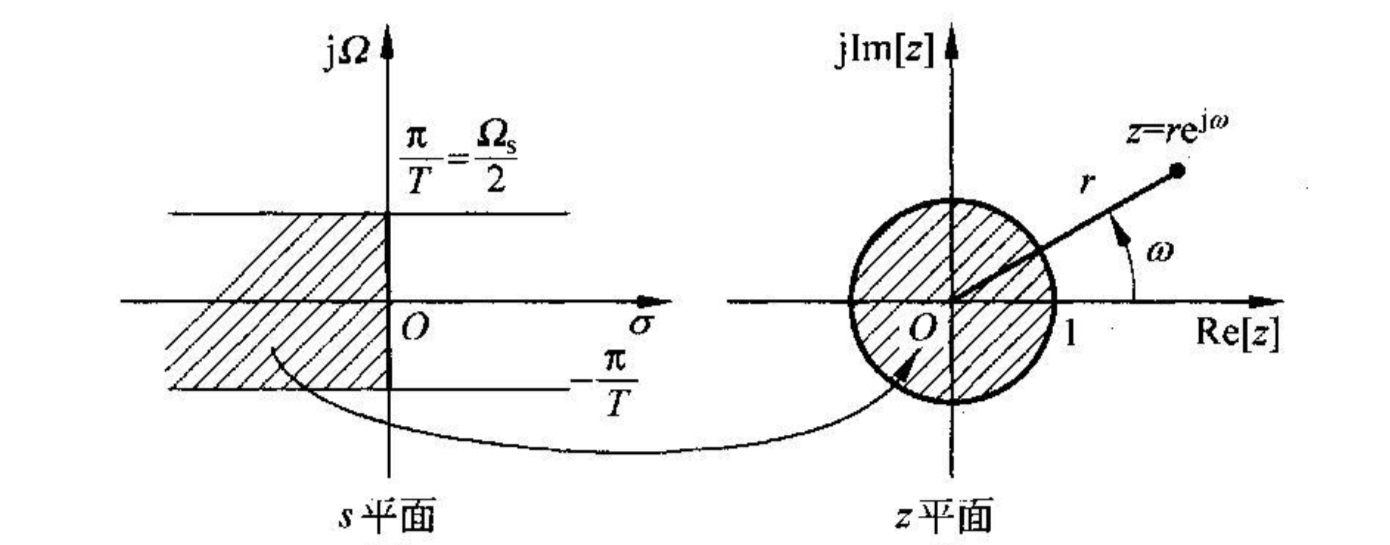
\includegraphics[width=\linewidth]{figure/IMG_48876557BC44-1.jpeg}
\end{figure}
\vspace{-15pt}

\item[DTFT] 单位圆上的Z变换
\(\mathcal F[x[n]] = X(e^{j\omega}) = \sum_{n=-\infty}^{+\infty} x[n] e^{-jn\omega}\)
\(x[n] = \frac{1}{2\pi} \int_{-\pi}^{\pi} X(e^{j\omega})e^{jn\omega}\D\omega\)

\{1,2,3,4,5,6,7\},N=5,\{7,9,3,4,5\}

\vspace{-10pt}
\begin{figure}[H]
    \centering
    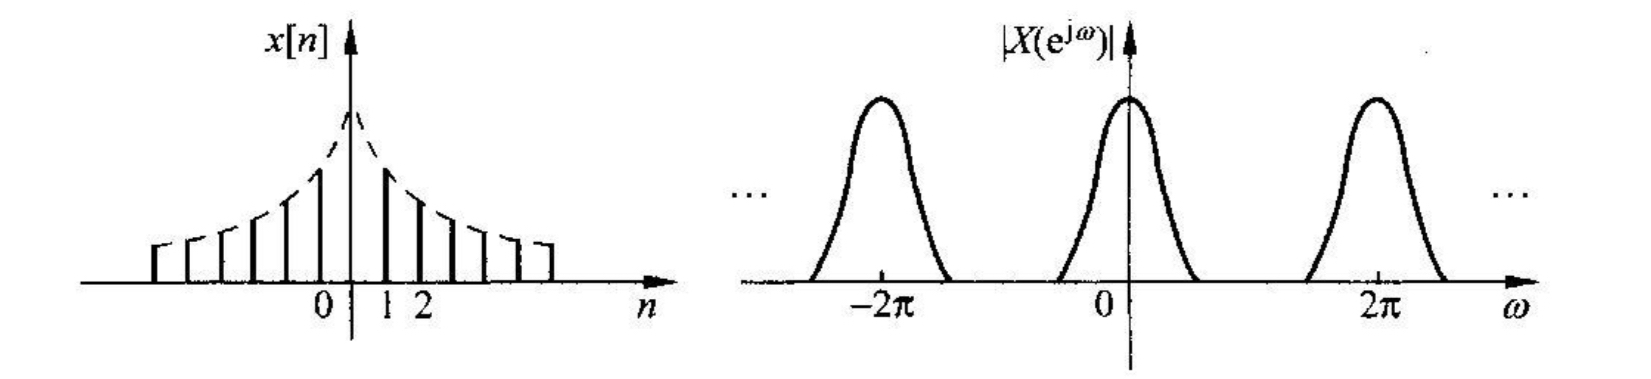
\includegraphics[width=\linewidth]{figure/IMG_CC52E79B1DEA-1.jpeg}
\end{figure}
\vspace{-20pt}

\end{description}


\subsection{系统函数}
\vspace{2pt}
\(H(z)=\frac{Y(z)}{X(z)}\quad h[n]\leftrightarrow H(z)\)

\vspace{-10pt}
\begin{table}[H]
    \tiny
    \setlength{\parskip}{0pt plus 0.5ex}
    \begin{tabular}{@{}ccc@{}}
    \toprule
    $h(t)$|$h[n]$ & $H(s)$ 极点 & $H(z)$ 极点 \\ \midrule
    衰减              & 左半平面        & 单位圆内        \\
    阶跃              & 原点          & 单位圆实轴交点    \\
    等幅震荡            & 虚轴,共轭       & 单位圆上,共轭     \\
    增长              & 右半平面        & 单位圆外        \\
    直流              & 实轴          & 正实轴         \\ \bottomrule
    \end{tabular}
\end{table}
\vspace{-10pt}

稳定系统:收敛域包含单位圆/虚轴\\
离散因果:\(z=\infty\)收敛(分子阶\(\leq\)分母阶)\\
连续因果:\(-\infty\)收敛,因果
因果稳定:极点全在单位圆内/左半平面

\vspace{-10pt}
\begin{table}[H]
    \tiny
    \setlength{\parskip}{0pt plus 0.5ex}
    \begin{tabular}{@{}cccc@{}}
    \toprule
    $h(t)$ & $H(s)$ 极点 & $H(z)$ 极点 & 稳定性 \\ \midrule
    衰减              & 左半平面        & 单位圆内        & 稳定  \\
    增长              & 右半平面        & 单位圆外        & 不稳定 \\
    增长              & 虚轴上多重极点     & 单位圆上多重    & 不稳定 \\
    等幅震荡            & 虚轴,共轭       & 单位圆上共轭     & 临界  \\
    阶跃              & 零点          & 单位圆实轴交点    & 临界  \\ \bottomrule
    \end{tabular}
\end{table}
\vspace{-10pt}


\vspace{-10pt}
\begin{figure}[H]
    \centering
    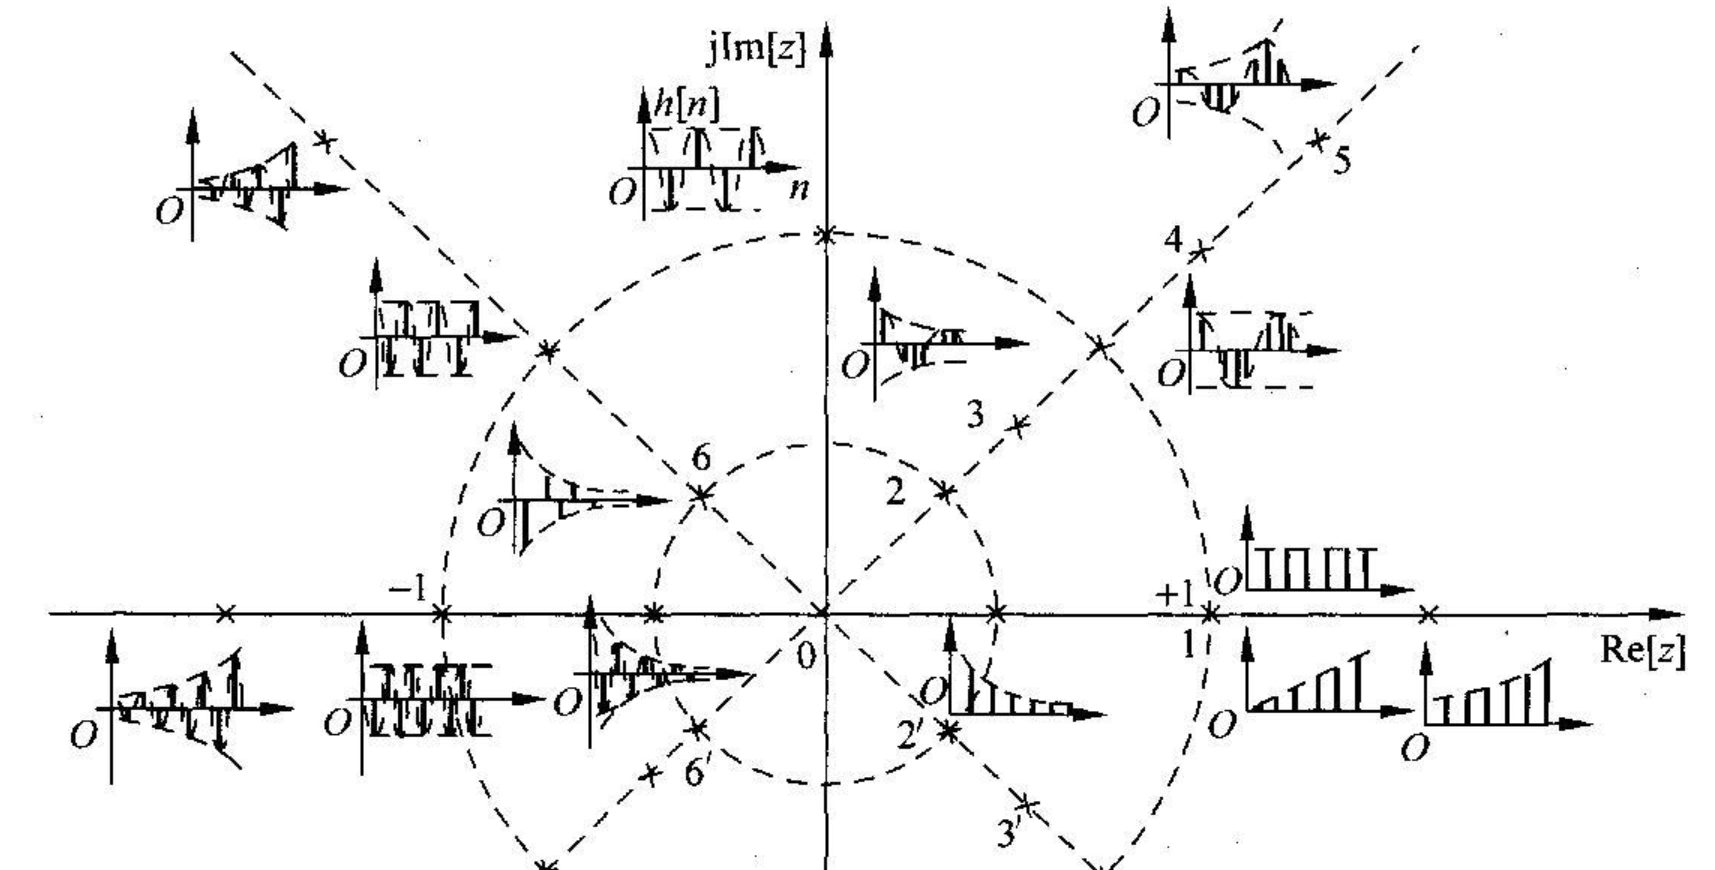
\includegraphics[width=\linewidth]{figure/Pasted image 20220612232835.png}
\end{figure}
\vspace{-10pt}
靠近原点振幅下降;向\(\pi\)运动频率上升。

\subsection{频率响应}

\(x[n] = e^{j\omega_0 n}\), \(y[n]=x[n]H(e^{j\omega_0})\),$H$ 的DTFT
\(H(e^{j\omega_0})=\|H(e^{j\omega_0})\|e^{j\varphi(\omega_0)}\),增益+相移

\vspace{-5pt}
\begin{description}
\tightlist
\item[几何确定] \(\left|\frac{H(e^{j\omega})}{K}\right| = \frac{\prod|\boldsymbol Z_j|}{\prod|\boldsymbol P_i|} = \frac{\text{零矢量模乘积}}{\text{极矢量模乘积}}\)
\(\varphi(\omega) = \sum \alpha_{z_j} - \sum \beta_{p_i} = \text{零矢幅角和} - \text{极矢幅角和}\)

\item[离散] 矢量终点 $\boldsymbol A$:$e^{j\omega}$,因此绕单位圆一周即可给出频响。(周期函数,$T=2\pi$)

\item[连续] \(H(j\Omega)\),矢量终点 $\boldsymbol A$ 从零点开始沿虚轴运动。$0\leq \Omega < \infty$

\end{description}

\subsection{相频特性}
单位圆内的零点,每转一圈,$\Delta\varphi(\omega) = 2\pi$\\
单位圆外的零点,每转一圈,$\Delta\varphi(\omega) = 0$

最小相位:唯一。\(M\)零点,\(2^M\)个同幅频特性。
\begin{description}
\tightlist

\item[全通]\(H_{ap}(z) = \frac{z^{-1}-z_0^*}{1-z_0z^{-1}}\)

连续:零极点分别位于虚轴左右,关于虚轴对称

\item[最小相位] 单位圆外/右半平面无零点 \\
每个周期内相频特性变化为零;
可以和全通系统级联表示非最小相位系统;
可逆;无负调现象。

\item[因果最小相位] 加上极点全在单位圆/左半平面

\vspace{-10pt}
\begin{figure}[H]
    \centering
    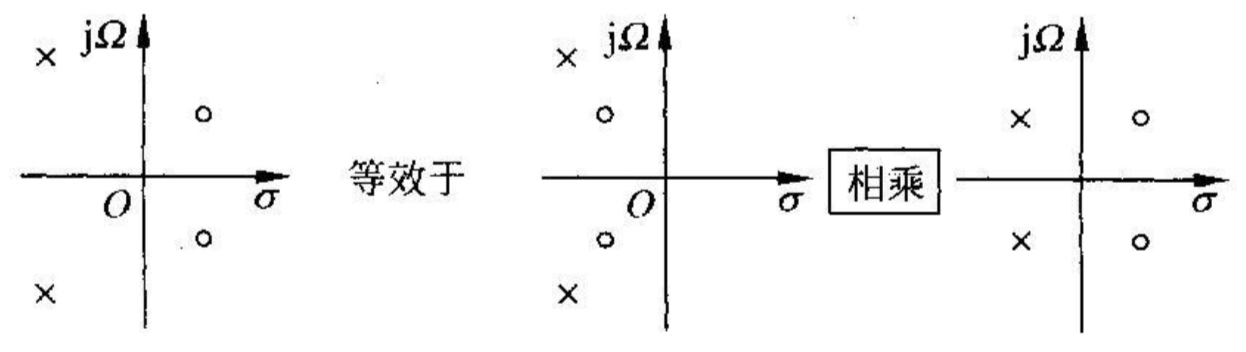
\includegraphics[width=\linewidth]{figure/IMG_EB82E9BC56FA-1.jpeg}
\end{figure}
\vspace{-10pt}
\end{description}
\vspace{-10pt}

% \vspace{-10pt}
% \begin{description}
% \tightlist
% \item[] 
% \end{description}
\section{FFT}
\subsection{DFT}
\(\operatorname{DFS}[\tilde{x}[n]]=\widetilde{X}[k]=\sum_{n=0}^{N-1} \tilde{x}[n] W^{n k}\)
\(\operatorname{IDFS}[\widetilde{X}[k]]=\tilde{x}[n]=\frac{1}{N} \sum_{k=0}^{N-1} \widetilde{X}[k] W^{-n k}\)

\(\displaystyle \operatorname{DFT}[x[n]]=X[k]=\sum_{n=0}^{N -1} x[n] W^{n k}, 0 \leq  k \leq  N-1\)
\(\displaystyle \operatorname{IDFT}[X[k]]=x[n]=\frac{1}{N} \sum_{k=0}^{N-1} X[k] W^{-n k}\)
\(W_N=W=e^{-j\,\frac{2\pi}{N}}\)

矩阵序列:\(R_N[n]=1,n\in [0,N-1]\)

\textbf{数据采样参数}\\
采样时间间隔:\(T_s=\frac{1}{f_s}<\frac{1}{2f_{\max}}\)\\
采样总时间:频率分辨率\(f_1\),\(T_1\geq\frac{1}{f_1}\)\\
采样数据点:\(N=\frac{T_1}{T_s}\),向上取到\(2^n\)\\

\vspace{-10pt}
\begin{figure}[H]
    \centering
    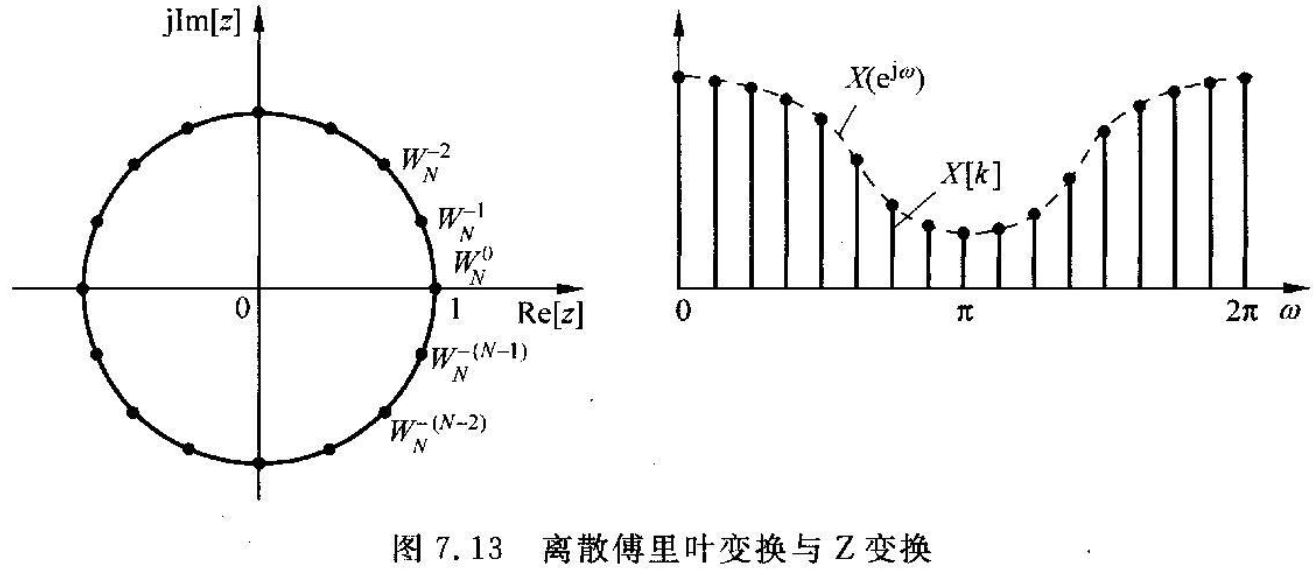
\includegraphics[width=\linewidth]{figure/Pasted image 20220611024619.png}
\end{figure}
\vspace{-10pt}

\subsection{圆卷积}
$x[n] (N) y[n] =\sum_{m=0}^{N-1} x[m]y((n-m))_N R_N[n]$\\
取反,取主值,相乘,叠加。\\
需要序列长度相等,补零。
\vspace{-10pt}
\begin{table}[H]
    \tiny
    \setlength{\parskip}{-2pt plus 0.5ex}
    \begin{tabular}{@{}cccccccl@{}}
    1 & 2 & 3 & 4 & 5 & 0 & 0 &     \\ \cmidrule(r){1-7}
    5 & 0 & 0 & 4 & 3 & 2 & 1 & =36 \\
    4 & 5 & 0 & 0 & 3 & 2 & 1 & =29 \\
    \end{tabular}
\end{table}
\vspace{-10pt}

圆卷积=线卷积:都补零到 $L=N+M-1$

\subsection{DFT性质}

\begin{description}
\tightlist
\item[线性] $ax[n]+by[n]\leftrightarrow aX[k]+bY[k]$

\item[圆移位] $x((n-m))_NR_N[n]\longleftrightarrow W^{mk}X[k]$
$x[n]\longrightarrow x((n-m))_NR_N[n]$ 右移\(m\)

\item[频域圆移位]
$W^{nl}x[n]\longleftrightarrow X((k+l))_NR_N[k]$

\item[频域圆卷积]
$Y[k] = \frac{1}{N}X[k](N)H[k]$
\end{description}
\vspace{-10pt}
\begin{figure}[H]
    \centering
    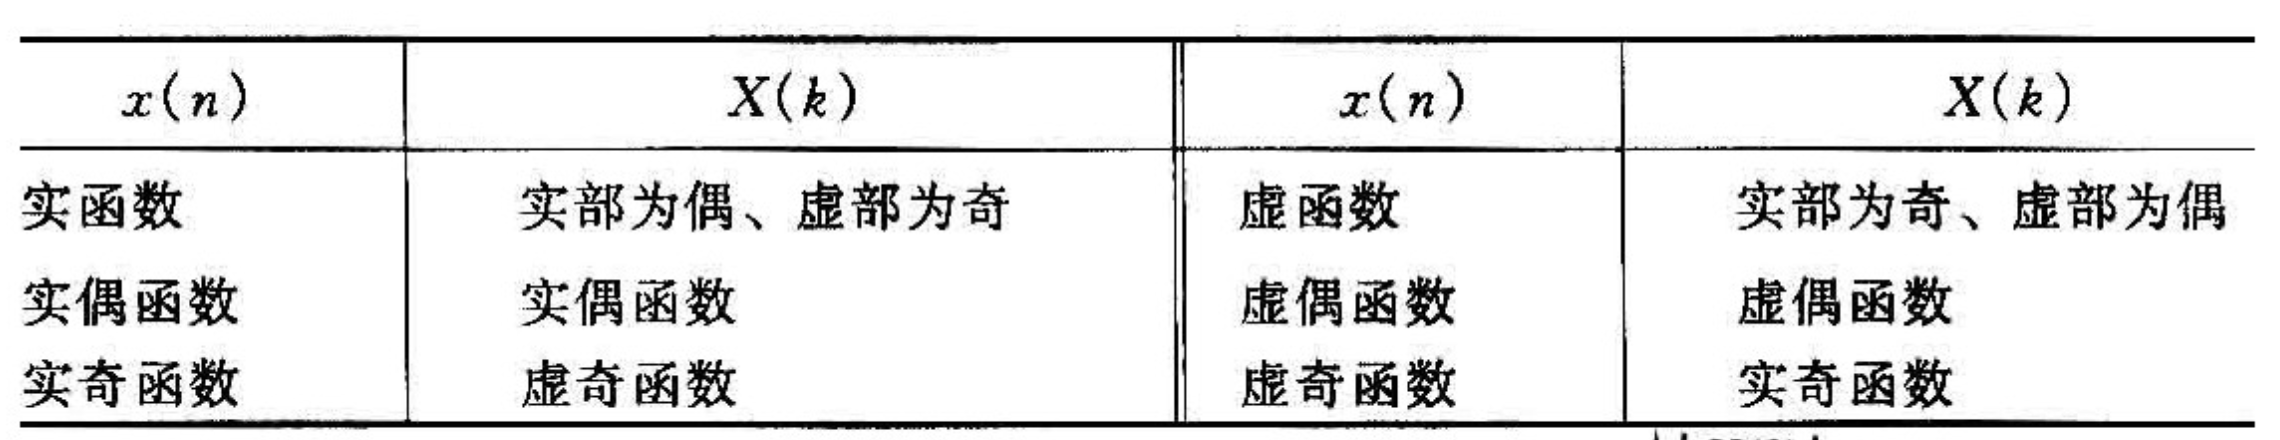
\includegraphics[width=\linewidth]{figure/dft.png}
\end{figure}
\vspace{-10pt}



\subsection{FFT}

DFT:每计算一个 $X[k]$,需要 $N$ 次复数乘法和 $N-1$ 次复数加法;需要算 \(N\) 个。

FFT:
复数乘法:\(\frac{N}{2}\cdot \log_2{N}\)\\
复数加法:\(N\cdot \log_2N\)

\subsection{快速卷积}
线:\(M\times N\); \((M-1)(N-1)\)

FFT:\(L\geq M+N-1\),取\(2^n\)\\
\(3\times\frac{L}{2}\log_2{L}+L\); \(3\times L\log_2{L}\)


\vspace{-10pt}
\begin{figure}[H]
    \centering
    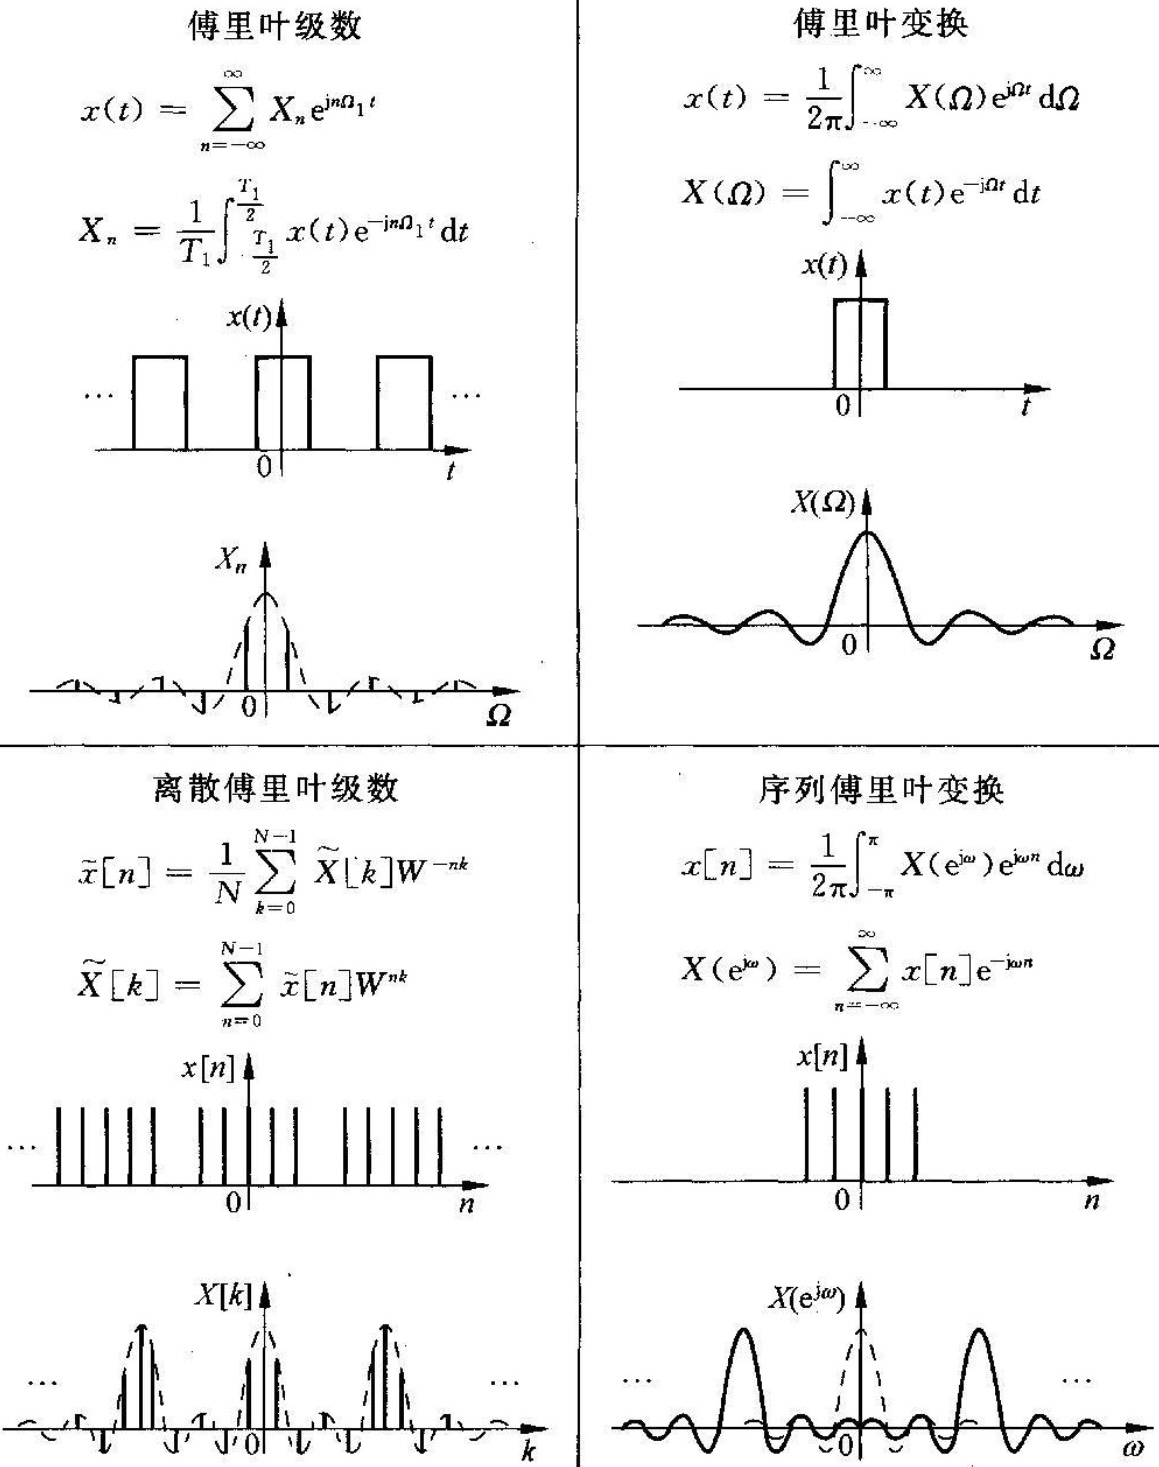
\includegraphics[width=\linewidth]{figure/Pasted image 20220611010632.jpg}
\end{figure}
\section{滤波器}
离散\(\|H(e^{j\omega})\|\)偶函数\(T=2\pi\),类型看\([0,\pi]\)

可实现性:\(\int_{-\infty}^{+\infty}|H(j\Omega)|^2<\infty\)

\subsection{IIR设计}
框图:\(H(z)\)上面是输入,下面是输出

脉冲响应不变:拉普拉斯反变化后采样,随后 z 变换
$H(s)\to h(t)\to h[n]\to H(z)$\\
适用部分分式,由于混叠,不适用高通。\\
\(\frac{1}{s-p_k}\to \frac{1}{1-e^{p_kT}z^{-1}}\)

双线性:令\(s=\frac{2}{T}\cdot \frac{1-z^{-1}}{1+z^{-1}}\)

\subsection{FIR设计}
通带频率 $\omega_{p}$, 截止频率$\omega_{s}$ 阻带衰减比率$A dB$\\
归一化频率: $\Omega=\frac{2 \pi \omega}{\omega_{s}}$, 其中 $\omega_{s}$ 为采样频率\\
(1) 选择理想低通滤波器的带宽: $\Omega_{1}=\frac{\Omega_{s}+\Omega_{p}}{2}$\\
(2) 根据衰减比率选择合适的加窗窗口;\\
(3) 根据过渡带 $\Omega_{2}=\Omega_{p}-\Omega_{s}$ 确定滤波器的长度: $N=\frac{2 \pi}{\Omega_{2}} \times R_{w}$,其中 $R_{w}$ 是加窗对应的过渡带宽度系数;\\
(4) $ h_{d}(n)=\frac{\sin \left[\Omega_{1}(n-a)\right]}{\pi(n-a)} \cdot W[n] $\\
其中
$a=N/2$,
$W[n]$是窗口函数
\section{总结}

这一学期的课程让我收获良多。但由于参与了2022北京冬奥会及冬残奥会,我在4月6日才解除隔离返回学校。赛事服务期间的课程由于时间可能会产生冲突,我都是利用学堂在线的MOOC课程进行学习的。在学习过程中,我感觉MOOC的内容编排上提前介绍的内容太多,不是很“循序渐进”。比如第一章的系统分类,一下子摆出了所有的分类类型,一时间信息量有些过于庞大。我认为郑教授的书的处理方法会比较适合自学,第一章先介绍一小部分系统分类,剩下的留到第二章线性时不变系统的时候统一介绍。或许MOOC因为回放方便的特性,会被认为比较适合在短时间内讲述结构性强,知识密度高的内容,但我认为MOOC另一个重要的方面是方便同学们进行自学,也有必要考虑知识点引入的循序渐进。以上是我关于MOOC课程的一些小想法。

另外由于4月6日前未能参与课堂教学环节(有学校的假条),还得麻烦卓大大留意一下我的课堂参与分数。我也会在考试后单独联系您,看看怎么处理这一部分分数~

\rule{0.3\linewidth}{0.25pt}
\scriptsize

Copyright \copyright\ 2022 陈辰

自04班 2020011633 chen-che20@mails.tsinghua.edu.cn

\tiny\url{CalaW/SignalsAndSystem-CheetSheet}


\vspace{-10pt}
\begin{figure}[H]
    \centering
    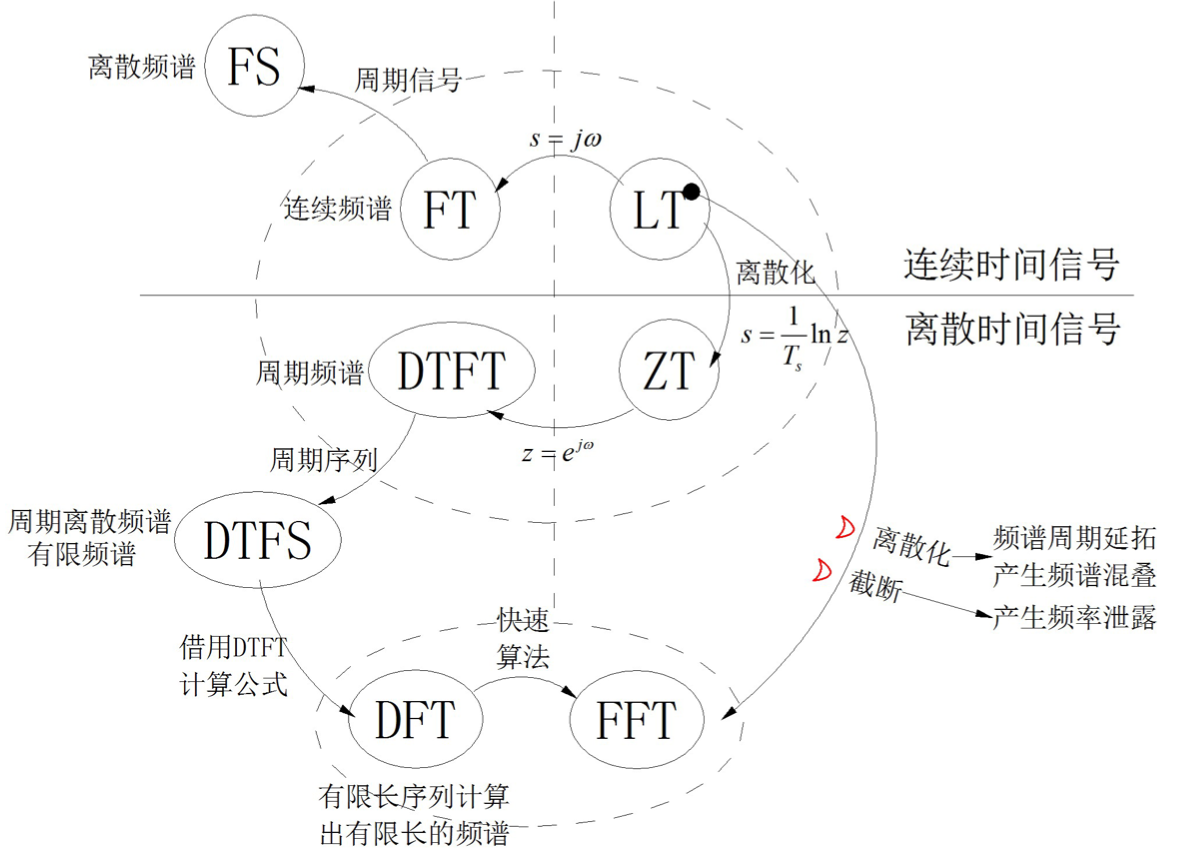
\includegraphics[width=2\linewidth]{figure/sum.png}
\end{figure}
\end{multicols*}
\end{document}
